\chapter{Design and Implementation}
\label{chap:implementation}

In this chapter the design and implementation of the prototype for the Austrian parliament is described. First of all, in Section \ref{sec:architecture} the overall architecture and the different components are being discussed. The more detailed description of the implementation is divided into four sections: Section \ref{sec:data_extraction_transforming} which shows how the protocols were accessed and transformed into structured data, section \ref{sec:export_db} which discusses the database export, section \ref{sec:analysis} which describes which analysis is done over the available data and section \ref{sec:visualization} which shows how the information gets displayed.

\section{Architecture}
\label{sec:architecture}
Figure \ref{fig:general_architecture} shows the general architecture of the prototype which was implemented. The ETL-Application brings the data from the protocols in the database whereas the web server application visualizes the results and shows statistics and graphs for the given data. The ETL-Application is implemented using the ETL pattern. This means that there are three distinct steps: Extract - Transform - Load. First the application reads an RSS feed which contains all the protocols for one legislative period (Extract). The retrieved HTML-files get parsed and are transformed into Java objects (Transform) which get loaded into a relational database\footnote{in the prototype, a PostgreSQL database was used} (Load). To visualize the then available data, the analysis engine queries the database, preforms analysis on it and converts the data in a form which can be displayed (e.g. a graph structure). Furthermore, this data is made available via RESTful web services. The Polymer web application accesses these web services and shows graphs and statistics. All the components will be described in more detailed in the later sections.

\begin{figure}
	\centering
	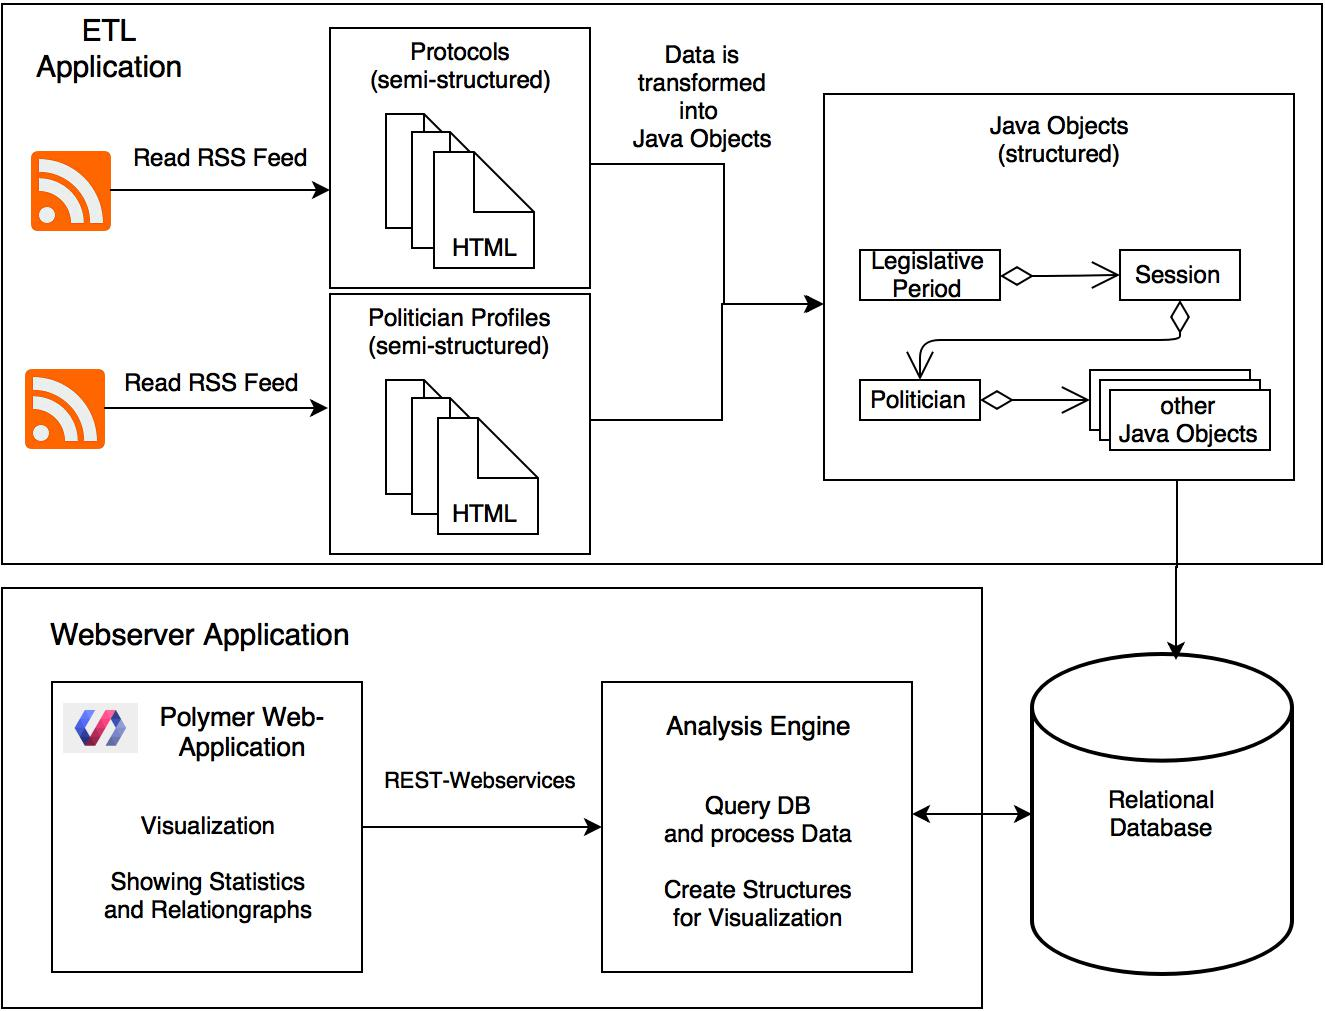
\includegraphics[width=\textwidth]{imgs/overall_architecture}
	\caption{General Architecture}
	\label{fig:general_architecture}
\end{figure}

\section{Data Extraction and Transforming}
\label{sec:data_extraction_transforming}
The first step which has to be done in the ETL-Application is the extraction. The data which should be transformed has to be collected and stored. In our case the data is contained in the stenographic protocols of the national council and politician profiles. Both the protocols and politician profiles are publicly available and can be found at the website of the Austrian parliament (See \url{https://www.parlament.gv.at/PAKT/STPROT/} and \url{https://www.parlament.gv.at/WWER/PARL/}). Furthermore, the protocols are available in PDF-format and since the $20^{th}$ legislative period also in HTML. As the transforming of the PDF-files would not result in sufficient quality, in this thesis only the HTML-files (the data since the $20^{th}$ legislative period) is being extracted and analyzed.

To collect the needed files automatically RSS feeds are used. This feed shows a list of the protocols of a specific legislative period. The application reads the feed and downloads all the protocols of the period. Then the content of each of the files get transformed into Java objects. To be able to understand the transformation process the structure of the file has to be clear. 

\section{Export into Database}
\label{sec:export_db}

\section{Analysis}
\label{sec:analysis}

\section{Visualization}
\label{sec:visualization}
